In het volgende hoofdstuk is zijn de lasten van de moonrover bepaald. Op basis van deze gegevens kunen we de juiste motor gaan selecteren voor de moonrover. Door de leverancier "Maxon" is er een advies gedaan van een reeks motoren en transmissies;
\begin{align*}
        motor: &RE25 1187xx\\
        transmissie: &Planetary Gearhead GP xx xx
\end{align*}
In dit hoofdstuk zullen wij een keuze gaan maken voor een specifieke motor in combinatie met een specifieke transmissie.


\subsection{Motorkeuze}
Binnen de aangegeven maxon reeks hebben wij gekozen voor de RE25 118745. In theorie is het mogelijk om elke motor te kieze binnen de aangegeven reeks in combinatie met de juiste transmissie. Voor deze specifieke situatie hebben we gekozen voor de RE25 118745. Dit is een wat kleinere motor binnen de reeks, echter is het mooie van deze motor dat hij een efficientie van 90 heeft. In afbeelding \ref{fig:RE25_118745} is te zien hoe de koppel toeren karakteristiek van de motor zich weerhoud tegen de last. In combinatie met de juiste transmissie kan deze motor goed ingezet worden bij de moonrover. In Bijlage \ref{app:datasheet motor} is de datasheet te zien van deze motor.
\begin{figure}[H]
        \centering
        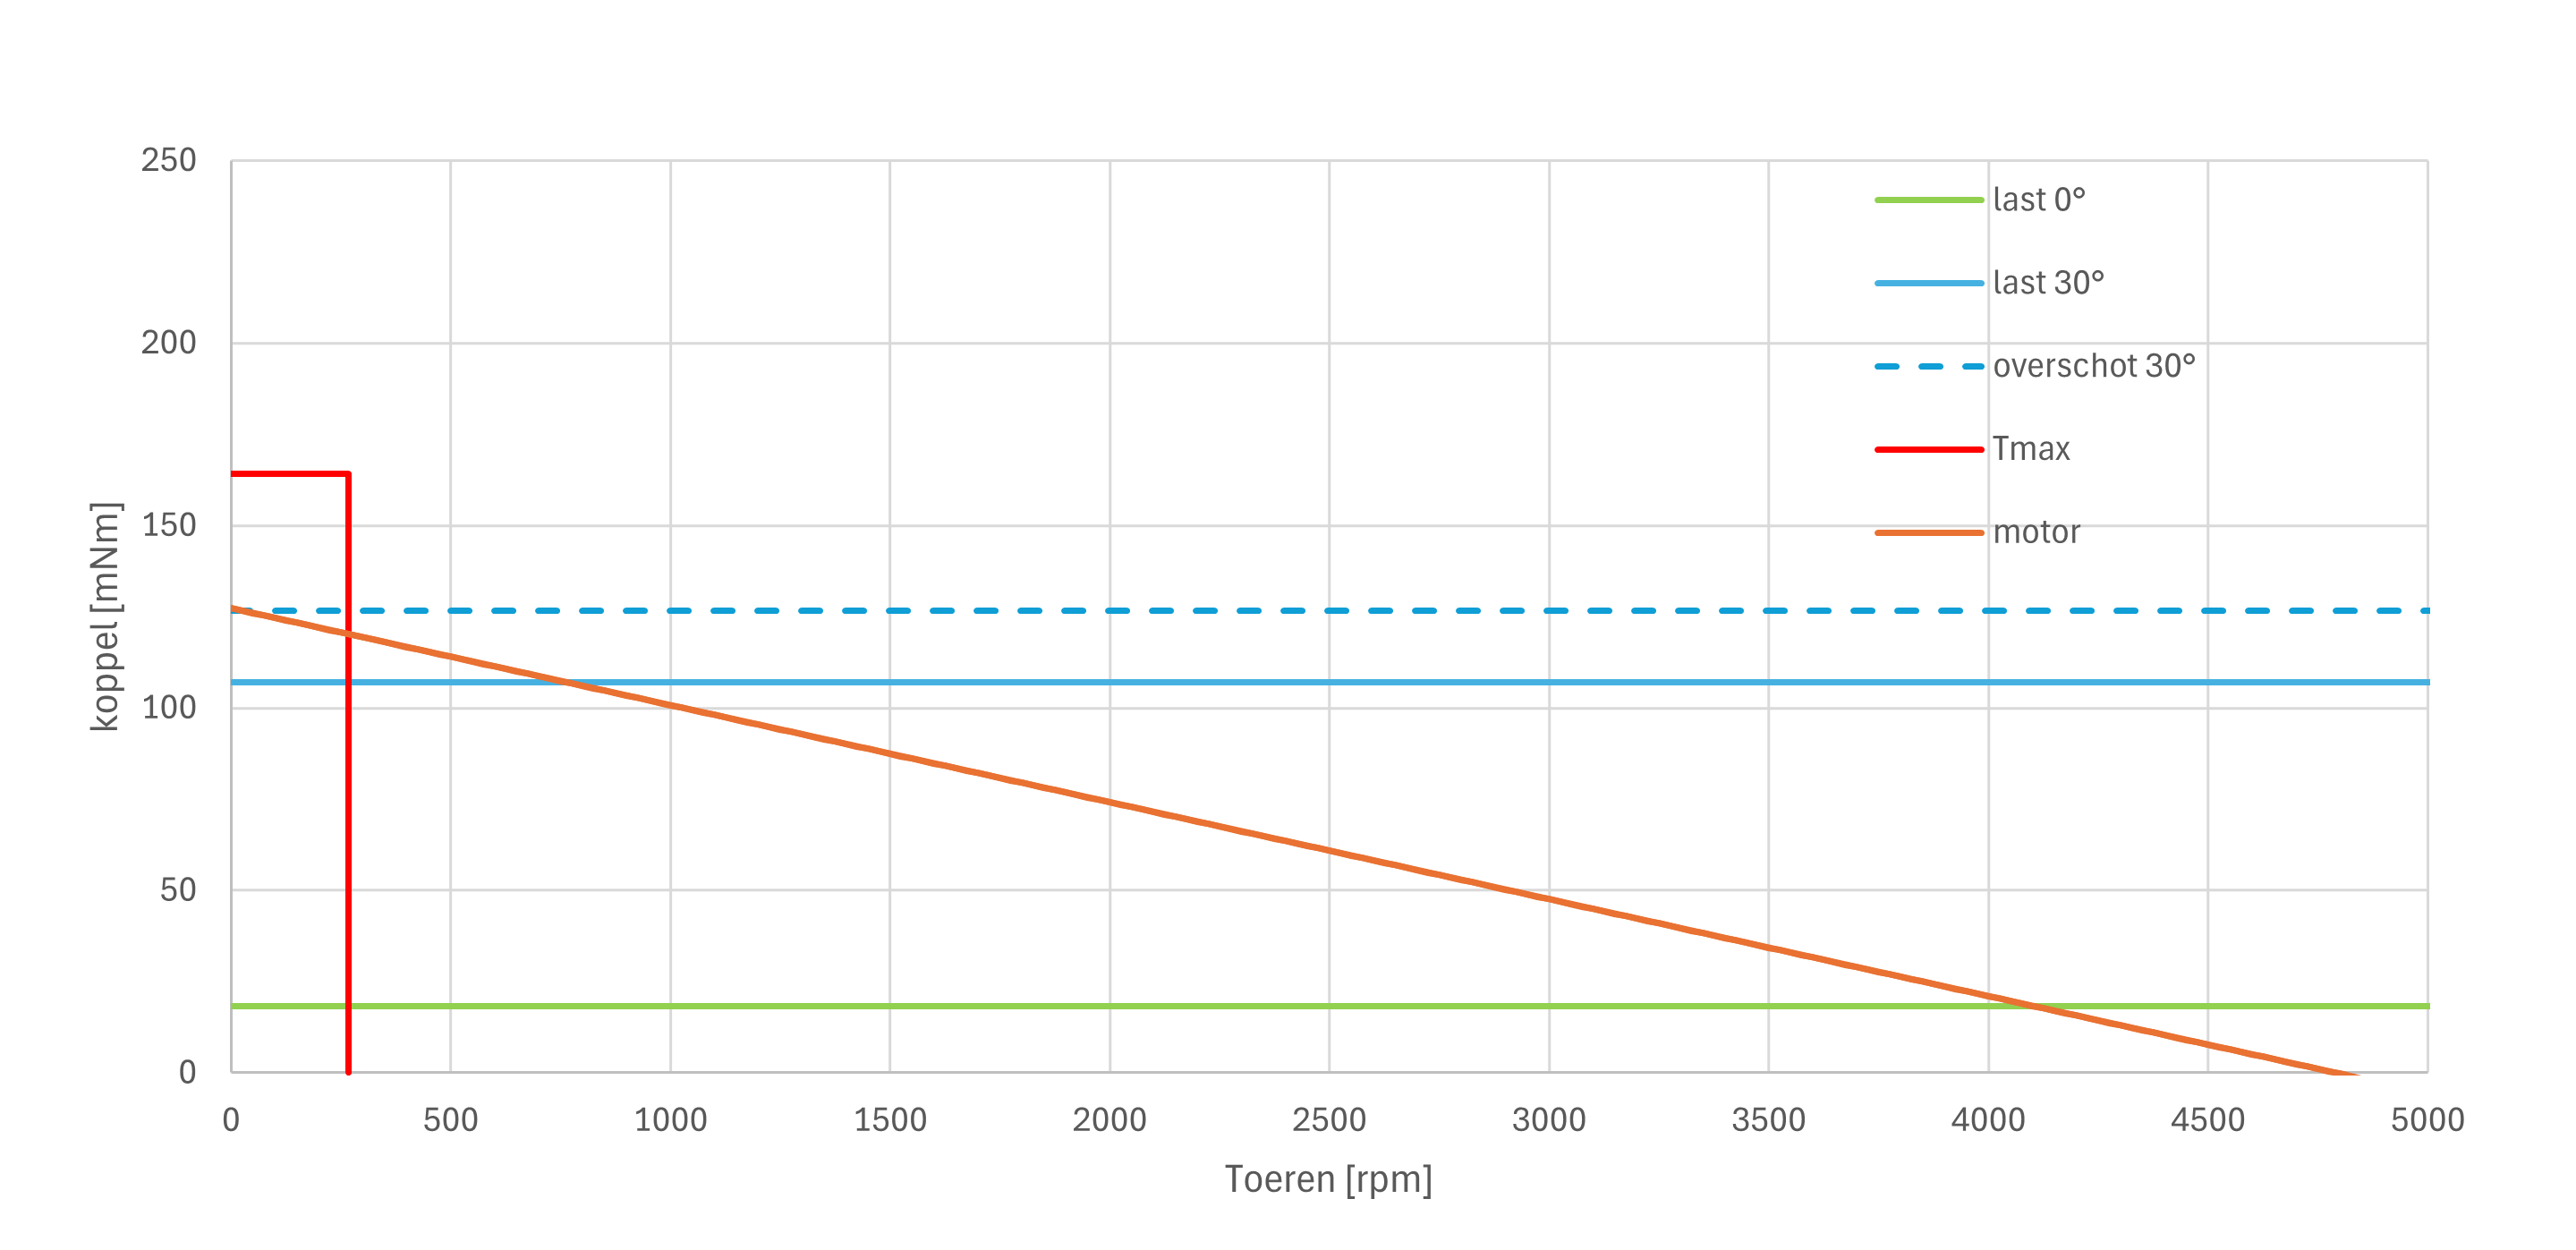
\includegraphics[scale=0.7]{RE25_118745.png}
        \caption{koppel toeren karakteristiek RE25 118745}
        \label{fig:RE25_118745}
    \end{figure}

\subsection{transmissiekeuze}

\subsection{efficientie}



\subsection{Warmtedisipatie}

Voor de moonrover zullen de motoren geleverd worden van het merk Maxon. Maxon heeft aangegeven dat zij de gekozen motor "maan bestendig" zullen maken. Hierbij zal ook rekening gehouden met de temperatuur verschillen op de maan en de warmte dissipatie hiervan. 

\subsection{Conclusie}